\textbf{Trees} are a kind of recursive data structure. Each tree has a \textbf{root label} (which is some value) and a sequence of \textbf{branches}. Trees are ``recursive'' because the branches of a tree are trees themselves! A typical tree might look something like this: 

\begin{center}
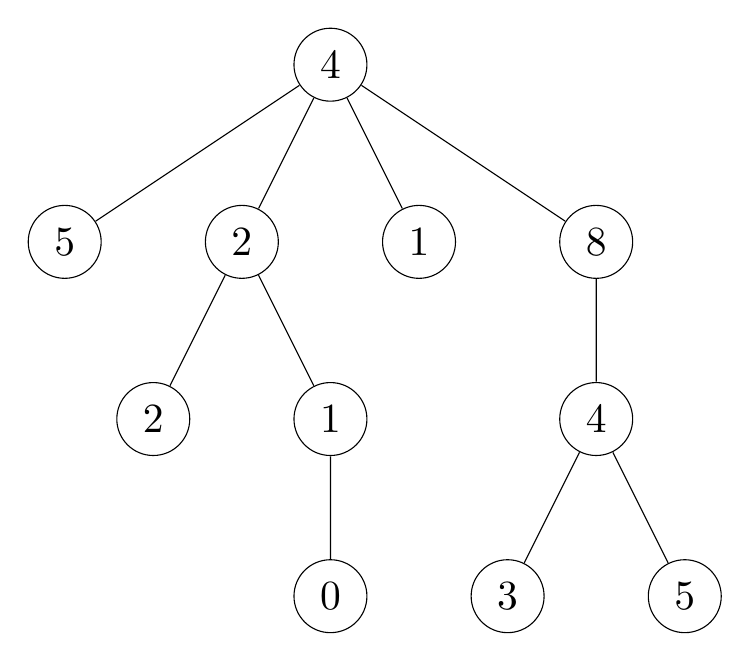
\begin{tikzpicture}[scale=1.5, transform shape]
    \node [circle, draw] (z){$4$}
        child {node [circle, draw] (a) {$5$}}
        child {node [circle, draw] (b) {$2$}
            child {node [circle, draw] (e) {$2$}}
            child {node [circle, draw] (f) {$1$}
                child {node [circle, draw] (h) {$0$}}
            }
        }
        child {node [circle, draw] (c) {$1$}}
        child {node [circle, draw] (d) {$8$}
            child {node [circle, draw] (g) {$4$}
                child {node [circle, draw] (i) {$3$}}
                child {node [circle, draw] (j) {$5$}}
            }
        };
\end{tikzpicture}
\end{center}
This tree's root label is $4$, and it has 4 branches, each of which is a smaller tree. The $6$ of the tree's \textbf{subtrees} are also \textbf{leaves}, which are trees that have no branches. 

Trees may also be viewed \textbf{relationally}, as a network of nodes with parent-child relationships. Under this scheme, each circle in the tree diagram above is a node. Every non-root node has one parent above it and every non-leaf node has at least one child below it. 

Trees are represented by an abstract data type with a \lstinline{tree} constructor and \lstinline{label} and \lstinline{branches} selectors. The \lstinline{tree} constructor takes in a label and a list of branches and returns a tree. Here's how one would construct the tree shown above with \lstinline{tree}: 

\begin{lstlisting}
tree(4,
    [tree(5),
     tree(2,
        [tree(2),
         tree(1,
            [tree(0)])]),
     tree(1),
     tree(8,
        [tree(4,
            [tree(3), tree(5)])])])
\end{lstlisting}

The implementation of the ADT is provided here, but you shouldn't have to worry about this too much. (Remember the abstraction barrier!)

\begin{lstlisting}
def tree(label, branches=[]):
	return [label] + list(branches)

def label(tree):
	return tree[0] 

def branches(tree):
	return tree[1:] # returns a list of branches
		
	\end{lstlisting}

Because trees are recursive data structures, recursion tends to a be a very natural way of solving problems that involve trees. 
\begin{itemize}
	\item The \textbf{recursive case} for tree problems often involves recursive calls on the branches of a tree. 
	\item The \textbf{base case} is often reached when we hit a leaf because there are no more branches to recurse on. 
\end{itemize}


\begin{guide}
	\textbf{Teaching Tips}
	\begin{itemize}
			\item Please make sure to check in with your students before mini-lecture so that you don't go over too much content that that they already feel comfortable with. 
			\item While it is typically true that your make the recursive calls on the branches of a tree and stop recursing when you reach a leaf, this is by no means always true, and you should make it clear that there will be exceptions to this rule of thumb. 
			\item Common Misconceptions:
			\begin{itemize}
				\item Students often have trouble with the idea that branches is a list of trees. Try to be specific when explaining, focusing on types. (Branches are lists, saving trees in them.)
				\begin{itemize}
					\item Try using the tree functions to build up different trees.
					\item Write out all the functions on the board and clearly define the types of the output and input.
				\end{itemize}
				\item Data Abstraction and Trees
				\begin{itemize}
					\item Although \lstinline{t[0]} returns the label from the tree, students should be using \lstinline{label(t)}. This is because \lstinline{t} is not a list, it is a tree which is a data abstraction!
					\item It’s important to explain why indexing branches (e.g. \lstinline{branches(t)[0]}) doesn't violate an abstraction barrier (since branches returns a list of trees).
				\end{itemize}
			\end{itemize}
			\item The objectives for students are to:
			\begin{itemize}
				\item Draw trees as graphical representations given Python code
				\begin{itemize}
					\item Mention to students that empty branches \lstinline{[]} is the default argument, so \lstinline{tree(5)} is the same as \lstinline{tree(5, [])}.
					\item Emphasize variable types.
					\item It may be helpful to mark pairs of parentheses to help in understand the nesting relationships.
					\begin{itemize}
						\item Branches is a function that returns a list of trees.
						\item Label values are numbers.
					\end{itemize}
				\end{itemize}
				\item Construct Python code given a graphical representation of a tree
			\end{itemize}
	\end{itemize}
\end{guide}
